% CS 455, SP'22 Software Design Document template
% Software design template based on the template from
% https://tex.stackexchange.com/questions/42602/software-requirements-specification-with-latex
%
\documentclass[letterpaper,12pt,oneside,listof=totoc]{scrreprt}
\usepackage{listings}
\usepackage{underscore}
\usepackage{longtable}
\usepackage{graphicx}
\usepackage[bookmarks=true]{hyperref}
\hypersetup{
    bookmarks=false,                                % show bookmarks bar
    pdftitle={Software Design Document}, % title
%    pdfauthor={Yiannis Lazarides},                  % author
%    pdfsubject={TeX and LaTeX},                     % subject of the document
%    pdfkeywords={TeX, LaTeX, graphics, images},     % list of keywords
    colorlinks=true,                                % false: boxed links; true: colored links
    linkcolor=blue,                                 % color of internal links
    citecolor=black,                                % color of links to bibliography
    filecolor=black,                                % color of file links
    urlcolor=purple,                                % color of external links
    linktoc=page                                    % only page is linked
}%
\def\myversion{1.0 }

\date{\today}
\author{} % suppress warning, do not fill this in
\begin{document}

% we don't use \maketitle because we overide the default title page here
\begin{titlepage}
\flushright
\rule{\textwidth}{5pt}\vskip1cm
\Huge{SOFTWARE DESIGN DOCUMENT}\\
\vspace{1.5cm}
for\\
\vspace{1.5cm}
Materials Ordering System\\
\vspace{1.5cm}
\LARGE{Release 1.0\\}
\vspace{1.5cm}
\LARGE{Version \myversion approved\\}
\vspace{1.5cm}
Prepared by Agents\\
\vfill
\rule{\textwidth}{5pt}
\end{titlepage}

\tableofcontents
% this will be automatically created from chapters, sections, and subsections

\listoffigures
% this will be automatically created from the figure environment

\listoftables
% this will be automatically created from the table environment

\chapter*{Revision History}
% Update this table for each revision of the requirements
% Add the new content followed by a \hline

\begin{tabular}{| c | p{0.60\textwidth} | p{0.30\textwidth} |}
\hline
Date     & Description   & Revised by \\
\hline
03/16/22 & Initial draft & Agents \\
\hline
03/23/22 & Initial draft & Agents \\
\hline
\end{tabular}

% What is a Software Design Document (SDD)?
%
% Software design is a process by which the software requirements are translated into a representation of software components, interfaces, and data necessary for the implementation phase. The SDD shows how the software system will be structured to satisfy the requirements. It is the primary reference for code development and, therefore, it must contain all the information required by a programmer to write code. The SDD is typically performed in two stages. The first is a preliminary design in which the overall system architecture and data architecture is defined. In the second stage -- i.e., the detailed design stage -- more detailed data structures are defined and algorithms are developed for the defined architecture.
%
% This template is an annotated outline for a software design document adapted from the IEEE Recommended Practice for Software Design Descriptions. The IEEE Recommended Practice for Software Design Descriptions have been reduced in order to simplify this assignment while still retaining the main components and providing a general idea.
%

\chapter{INTRODUCTION}

\section{Purpose}
This software design document describes the architecture and system design of the Agent. It will go into detail on the purpose, scope, architecture, the design of the data, the component design, and the requirements matrix.

\section{Scope}
%Provide a description and scope of the software and explain the goals, objectives and benefits of your project.
The purpose of this Project is allow Windows and Linux user to install Agent into their device. When running the software, Agents it will collect data of CPU usage, memory usage, disk usage, and service applications that are currently running. Those data will be send to a monitor Engine and get store in to a database. The end user will be allow to see those data report on a dashboard. The benefits of this software is to allow the user to track their hardware usage in real time. 


\section{Overview}
%Provide an overview of this document and its organization. 
This software design document will provide an overview design for the Agent. Design will start with the system overview, then went to detail of the architectural design. After architectural design the next step will be data design. Agent data Will be in JSON format. There will not be any human interface design for Agent. The end of the this document will have a requirements matrix where all the requirements for the Agent will be listed there.


\section{References}
%This section is optional. List any documents, if any, which were used as sources of information. (May not have any) :(
N/A

\section{Definitions and Acronyms}

%This section is optional. Provide definitions of all terms, acronyms, and abbreviations that the reader may need to know to properly understand this SDD. These definitions should be items used in the SDD that are most likely not known to the audience.
Table~\ref{Acronyms} describes acronyms that's in this document (Agent SDD).

\begin{table}[h!]
\centering
\begin{tabular}{| c | p{0.70\textwidth} |} 
\hline
Acronyms & Explication\\
\hline
SDD & Software Design Document\\
\hline
JSON & JavaScript Object Notation \\
\hline
TCP & Transfer Control Protocol\\
\hline
ACK & Acknowledged \\
\hline


\end{tabular}
\caption{Acronyms and Abbreviations}
\label{Acronyms}
\end{table}





\chapter{SYSTEM OVERVIEW}

The CS455 Monitor System is a network monitoring system that will monitor UNA's CS network in order to help users identify and address potential network problems as they occur. The system will automatically collect and store data, as well as provide warnings and error messages when certain events trigger, such as an unresponsive agent or disk is at capacity. However, the system will rely on users to see the messages and act on them; the system is \textbf{not} automated to handle the events. As a specific example, if an error message pertaining to an unresponsive agent appears, it is the user's job to determine why the connection has failed and handle the issue. The Monitor System contains four sub-systems working in tandem; Agents, Monitoring Engine, Data Store, and a Dashboard.

The monitoring system is relatively simple. Agents, installed on devices connected to the network, will collect basic usage statistics such as CPU usage, memory usage, disk usage, network usage, and service applications that are currently running on the device. The frequency at which to collect data will be specified in the configuration text file (though in cases where a time is not specified there is a default time). The configuration file will also associate each agent with a unique ID and name corresponding to the device it is installed on in order to keep track of the data associated as it transfers though the system as a whole. This configuration file also contains the host name of the Engine should the user decide to port the Engine to another device. Each agent will automatically send its collected data to the Monitoring Engine over the network to be stored in the Data Store.

The Monitoring Engine (or simply the Engine), hosted on the CS server, will take in data from the Agents, perform sanity checks on the data, and then pass it on to the Data Store for storage. A "sanity check" is ensuring that incoming data is in a logical range. For instance, it is impossible for CPU usage to be above 100\%. It is impossible for the disk usage to be above 120\%. It is impossible for memory usage to be a negative percent. Should the Engine receive invalid data such as this, it will log an error to the Data Store. The Engine also contains a configuration file that details the host name of the Data Store that can be changed should the user want to port the Data Store to another device. This configuration file also knows the frequency it should be getting updates from each Agent. If the Engine receives no update from an Agent after that configured time frame, it logs an error message to the Data Store. The user will never interact directly with the Engine.

The Data Store, also hosted on the CS server, will take data from the Monitoring Engine and sort it into one of two fundamental types of data, metrics or logs. Metrics are numerical values that describe some aspect of a system at a particular point in time. Logs contain different kinds of data organized into records with different sets of properties for each type. The user will never directly interact with the Data Store. The Data Store acts solely as a place to store collected metrics and logs. The Data Store will be scalable to store information of up to fifty active Agents, process queries from up to a dozen active Dashboards, and be able retain data for up to a year. Users are able to remove or archive specific data in the Data Store.

The Dashboard will provide easy access to viewing the metrics of multiple different devices. Users will be able to view both current and past metrics for a device as well as see if there are connection issues with an Agent's monitored device. 

%Give a general description of the functionality, context, and design of your project. Provide any background information if necessary. 


\chapter{SYSTEM ARCHITECTURE}

\section{Architectural Design}

%Develop a modular program structure and explain the relationships between the modules to achieve the complete functionality of the system. This is a high level overview of how responsibilities of the system are partitioned and then assigned to subsystems. Identify each high level subsystem and the roles or responsibilities assigned to it. Describe how these subsystems collaborate with each other in order to achieve the desired functionality. Don't go into too much detail about the individual subsystems. The main purpose is to gain a general understanding of how and why the system was decomposed, and how the individual parts work together. Provide a diagram showing the major subsystems and data repositories and their interconnections. Refer to and describe the diagram in the narrative. %Price Will Look At This.
The system is split into five modules. The first module is the CPU module. This module is responsible for accessing the system statistics of the CPU and returning it to the main driver. The next module in the system is the Disk module. The Disk module is in charge of taking statistics from the Disk of the system and send it to the main driver. The next module is the Memory module. It is in charge of taking the data from the memory of the system and sending the data statistics to the main driver. The next module is the Network module. It will take the network statistics of the system and return them to the main driver. Finally we have the TCP transfer module. This module is in charge of sending all of the data that is converted to a JSON to the next step of the system we are building.


\section{Decomposition Description}

%Provide a decomposition of each one of the subsystems in the architectural design. You may choose to give a functional description or an object oriented (OO) description. For a functional description use appropriate diagrams such as top-level data flow diagrams (DFD) and structured decomposition diagrams. For an OO description use the appropriate diagrams such as subsysterm model, object digrams, generalization diagram(s), aggregation diagram(s), interface, and specification diagrams. 
Currently building the subsystem module/object diagrams.
\begin{figure}
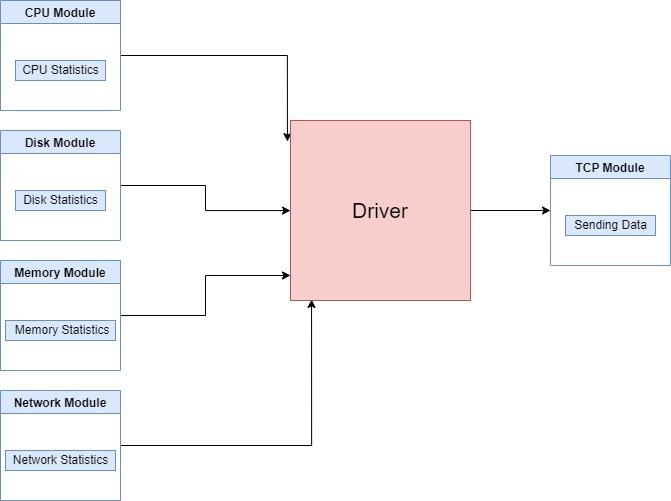
\includegraphics[width=15cm]{SDDChart.jpg}
  \caption{\label{fig:module} Agent System Design }
\end{figure}

\section{Design Rationale}

Discuss the rationale for selecting the architecture described in the previous section including critical issues and trade/offs that were considered. You may discuss other architectures that were considered, provided that you explain why you didn't choose them.


\chapter{DATA DESIGN}

\section{Data Description}
The data the Agent receives from the hardware comes in as four tuple variables. These variables are CPU, DISK, MEMORY, and NETWORK. These variables will be then added to a single JSON file on the system in the order of CPU, DISK, MEMORY, and NETWORK. That JSON file will then be sent out to the Engine.

The \textbf{CPU} data is organized as the percentage of time used in the last minute, ten minutes, and fifteen minutes.
The \textbf{Disk} is organized as total disk, used disk, free disk, and percentage used.
The \textbf{Memory} is organized as total memory, available memory, percent used, used, free, active, inactive, wired.
The \textbf{Network} is organized as bytes sent, bytes received, packets sent, packets received, error in, error out, drop in, and drop out.


%Explain how the information domain of your system is transformed into data structures. Describe how the major data or system entities are stored, processed and organized.

\section{Data Dictionary}

Alphabetically list the system entities or major data along with their types and descriptions. If you provided a functional description in the ``Decomposition'' Section, list all the functions and function parameters. If you provided an OO description, list the objects and the associated attributes, methods and method parameters.


\chapter{COMPONENT DESIGN}

%Give a detailed description of what each component does in a systematic way. If you gave a functional description in ``Decomposition'' section, provide a summary of your algorithm for each function using either a procedural description language (PDL) or pseudocode. If you gave an OO description, summarize each object's member functions for all the objects listed using PDL or pseudocode. Describe any local data when necessary. This section should include enough information for a competent programmer to implement each component. It should NOT be actual code.

Agent will have three major components. 
\begin{enumerate}
\item Environment check
    \begin{itemize}
        \item Agent will check for the device environment before collecting data.
        \item If the Agent wasn't in the correct environment, then Agent will not collect any data from this device.
    \end{itemize}
\item Data collection
    \begin{itemize}
        \item Agents it will collect data of CPU usage, memory usage, disk usage, and service applications that are currently running.
        \item After data collection, the data will be formatted into a JSON file.
    \end{itemize}
\item Data forward to Engine
    \begin{itemize}
        \item Data will be sent to the Engine using a TCP three way handshake where the Agent will send a message to the Engine. The Engine will send a ACK message back. Then the Agent will send the data over. 
    \end{itemize}


\end{enumerate}

The first component is to make use Agent is used in the correct environment(Windows and Linux). The second component will be collecting the data from the device. Finally, the last component will send the data collected over to Engine using JSON format. 


\chapter{HUMAN INTERFACE DESIGN}

Agent team is responsible for data collection only thus there will be no Human user interface.


\chapter{REQUIREMENTS MATRIX}

%Provide a cross-reference that traces each component and data structure to the requirement(s) in the SRS document. Use a tabular format to show which system components satisfy each one of the functional and non-functional requirements. Refer to the requirements by the number/code used in the SRS document.

\begin{longtable}{ p{0.10\textwidth} |  p{0.25\textwidth} | p{0.50\textwidth} }
    \hline
   \textbf{ID} & \textbf{Requirement} & \textbf{Functional Requirement} \\
    \hline
    SR20 & Agent runs on Windows & Verify all functionality of an Agent works on Windows OS.\\
    \hline
    SR21 & Agent runs on Unix-like & Verify all functionality of an Agent works on Unix-like OS.\\
    \hline
    SR03 & Agent can send valid data to Engine & Verify an Agent can send a data packet to the Engine over the network and receive an
    acknowledgement from the Engine in under 300 milliseconds. \\
    \hline
    
\caption{Requirements Matrix}
\label{ReqMatrix}
\end{longtable}


\end{document}
